% Mars Survival Map -- technical report (Red Circle team, NASA Space Apps 2026)
% Build: pdflatex report.tex (twice).  Every figure in this report comes from web/sources.json or the code in this repository.
\documentclass[11pt,a4paper]{article}
\usepackage[utf8]{inputenc}
\usepackage[T1]{fontenc}
\usepackage{lmodern}
\usepackage[margin=2.3cm]{geometry}
\usepackage{amsmath,amssymb}
\usepackage{booktabs,longtable,tabularx,array}
\usepackage{xcolor}
\usepackage{tikz}
\usetikzlibrary{arrows.meta,positioning,shapes.geometric,fit}
\usepackage{listings}
\usepackage{enumitem}
\usepackage[hidelinks]{hyperref}
\usepackage{url}
\usepackage{microtype}

\definecolor{leaf}{HTML}{4A9A2F}\definecolor{sky}{HTML}{2F9BE0}\definecolor{marsred}{HTML}{B8432A}
\definecolor{sun}{HTML}{F0BF2B}\definecolor{crimson}{HTML}{A1162F}\definecolor{ember}{HTML}{EC7A2C}\definecolor{violet}{HTML}{6A3FA8}
\definecolor{ink}{HTML}{1B2540}
\hypersetup{colorlinks=true,linkcolor=violet,urlcolor=sky,citecolor=violet}
\lstset{basicstyle=\ttfamily\footnotesize,breaklines=true,frame=single,rulecolor=\color{ink!25},backgroundcolor=\color{ink!3},columns=fullflexible,keepspaces=true}
\setlist{itemsep=2pt,topsep=3pt}
\newcommand{\hyp}[1]{\textcolor{marsred}{\textbf{[#1]}}}   % flags a hypothesis / team assumption
\renewcommand{\_}{\textunderscore\allowbreak}
\newcommand{\code}[1]{\texttt{#1}}
\emergencystretch=3em\setlength{\parindent}{0pt}\setlength{\parskip}{5pt}

\title{\textbf{Mars Survival Map}\\[2pt]\large Data sources, processing pipeline, algorithms and data structures\\[2pt]\normalsize Technical report -- NASA Space Apps 2026, challenge ``Interplanetary Survival Guide: Martian Map''}
\author{Red Circle team, Douala}
\date{\today}

\begin{document}
\maketitle
\begin{abstract}\noindent
Mars Survival Map is a static web application that answers one question: \emph{where, and how, can a person on foot survive on Mars?}
It works at three scales: a global screening grid (0.5$^\circ$, about 30~km), an overview of the whole Jezero region (20~m/px), and a detailed site map (metre scale)
with hazard classes, least-energy routes, a return-to-shelter reach, radio line of sight, shadows, a time budget and a simulated walker.
This report documents each data source, how it is preprocessed, every algorithm, and the data structures used. Values that come from measurements,
from published models, or from a team assumption are labelled as such throughout; \hyp{red tags} mark hypotheses that are not backed by a Mars measurement.
\end{abstract}
\tableofcontents

%------------------------------------------------------------------------------------------------
\section{Scope and ground rules}
\begin{itemize}
\item \textbf{Open data only.} Every dataset is downloadable without login or payment. Measurements are preferred; open, labelled models are allowed.
\item \textbf{Every number is traceable.} It comes from a source in \code{web/sources.json} (name, publisher, full URL, what was taken, use, status) or is declared a team assumption.
\item \textbf{Hypotheses are stated as hypotheses.} A quantity measured on Earth or the Moon and used on Mars (walking cost, suit power) is shown with the chip ``Physics model'' or ``Team assumption'' in the interface.
\item \textbf{Static deployment.} All heavy processing is done offline by Python scripts; the browser only reads precomputed binary files and runs light algorithms (routing, reach, line of sight, shadows) on the client. Hosting is a plain static folder (\code{web/}, Vercel).
\end{itemize}

%------------------------------------------------------------------------------------------------
\section{System architecture}
\begin{figure}[h]\centering
\resizebox{\textwidth}{!}{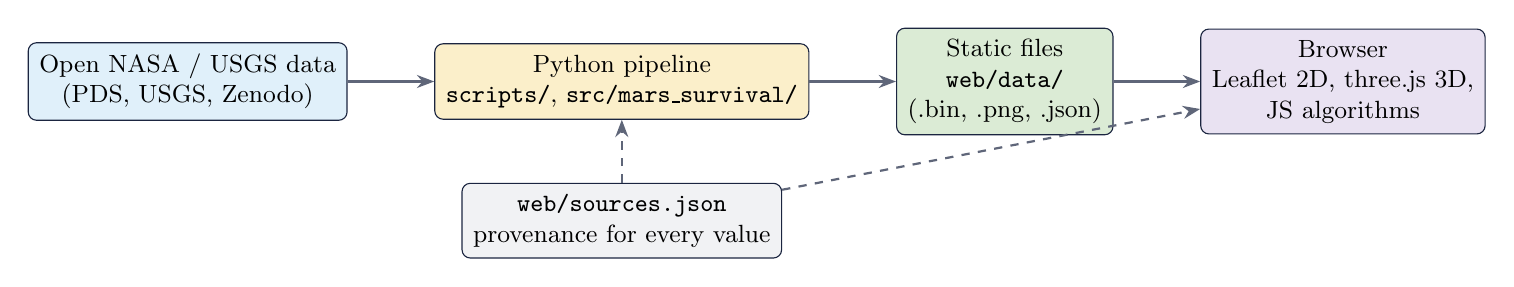
\begin{tikzpicture}[font=\small,node distance=9mm and 11mm,
 box/.style={draw=ink,rounded corners=3pt,fill=white,minimum height=8mm,align=center,inner sep=4pt},
 srcs/.style={box,fill=sky!15},procs/.style={box,fill=sun!25},outs/.style={box,fill=leaf!20},webs/.style={box,fill=violet!15},
 arr/.style={-{Stealth[length=2.2mm]},thick,ink!70}]
\node[srcs] (s1) {Open NASA / USGS data\\(PDS, USGS, Zenodo)};
\node[procs,right=of s1] (p1) {Python pipeline\\\code{scripts/}, \code{src/mars\_survival/}};
\node[outs,right=of p1] (o1) {Static files\\\code{web/data/}\\(.bin, .png, .json)};
\node[webs,right=of o1] (w1) {Browser\\Leaflet 2D, three.js 3D,\\JS algorithms};
\draw[arr] (s1)--(p1);\draw[arr] (p1)--(o1);\draw[arr] (o1)--(w1);
\node[box,below=8mm of p1,fill=ink!6] (t) {\code{web/sources.json}\\provenance for every value};
\draw[arr,dashed] (t)--(p1);\draw[arr,dashed] (t)--(w1);
\end{tikzpicture}}
\caption{Offline processing, static hand-over, client-side computation.}
\end{figure}

Three levels share the same palette and layout (two sidebars around a Google-Maps-style map):
\begin{description}
\item[Globe] (\code{globe.html}) global screening on a 0.5$^\circ$ grid. Real layers plus a partial score with a coverage figure per cell.
\item[Overview] (\code{overview.html}) the whole Jezero region at 20~m/px, with the detail windows drawn on it.
\item[Site] (\code{index.html}) a window a few km wide at metre-scale resolution (the current Jezero build is 4~m/px: a 4~km window block-averaged from the 1~m DTM); \code{index.html?site=<id>} opens another window stored in \code{web/data/sites/<id>/}.
\end{description}

%------------------------------------------------------------------------------------------------
\section{Data sources}
Table~\ref{tab:src} lists the sources used. The full registry (with exact files, licences and status) is \code{web/sources.json}, shown on \code{sources.html} and exported to \code{docs/ANALYSIS\_REPORT.md}.

\begin{table}[h]\centering\small
\begin{tabularx}{\textwidth}{@{}l>{\raggedright\arraybackslash}p{4.2cm}>{\raggedright\arraybackslash}X@{}}
\toprule
\textbf{Level} & \textbf{Source} & \textbf{What is taken / used for}\\\midrule
Site & HiRISE stereo DTM \code{DTEEC\_023524\_1985\_023379\_1985\_U01} (UA/HiRISE), $\approx$1~m/px, 700~MB &
 A window (6~km) read with HTTP Range requests; elevation $\to$ slope, roughness, hazard, routes, 3D mesh.\\
Overview & Mars 2020 Science Investigation CTX DEM mosaic (USGS Astrogeology, Calef 2021), 20~m/px, 87~MB, public domain &
 Whole-crater hillshade (lat 17.58--19.29, lon 76.99--78.58); display only, not used for routing.\\
Site & Mars 2020 MEDA bundle (NASA PDS Atmospheres), \code{CAL\_ATS}, \code{CAL\_PS} &
 Air temperature (kelvin) and pressure (pascal) per sol $\to$ mean temperature, day/night swing for the outing planner.\\
Globe & MGS MOLA elevation (USGS/GSFC), 463~m/px &
 Global elevation; pressure and radiation are derived from it.\\
Globe & Mars Odyssey GRS neutron tables (NASA PDS Geosciences) &
 Epithermal neutron flux as a hydrogen / water-ice proxy.\\
Globe & MGS TES thermal inertia &
 Surface thermal inertia (tiu).\\
Globe & MRO MCS temperature, processed by Wang \& Jin (2025) &
 Mean surface temperature and day/night swing per cell.\\
Globe & Mars Climate Database dust climatology &
 Dust opacity (7 Mars years), time-weighted.\\\midrule
Physics & Minetti et al. 2002, \emph{J.\ Appl.\ Physiol.} 93:1039 &
 Metabolic cost of walking vs.\ slope (Earth, 10 athletes, no load).\\
Physics & Cavagna, Willems \& Heglund 2000, \emph{J.\ Physiol.} 528:657 &
 Gravity dependence of the level-walking work (mechanical, 3 subjects, 0.4~g).\\
Physics & Apollo 16 Time and Motion Study (NASA MSC M72-6); NASA TN D-7883; NSSDC LRV ranges &
 Suit power ($\approx$326~W walking), mean 930~Btu/h, rover ranges 5.0/4.5/7.6~km.\\
Physics & Allison \& McEwen 2000 (Mars24 algorithm) &
 Local true solar time, equation of time, $L_s$.\\
Physics & NASA Mars Fact Sheet &
 Mean radius 3389.5~km, gravity, mean temperature 214~K.\\\bottomrule
\end{tabularx}
\caption{Data and physics sources (summary).}\label{tab:src}
\end{table}

\textbf{Honest gaps.} No NASA numeric slope limit for a walking suited human on Mars exists in the sources we found; the roughness thresholds (0.25/0.6/1.5~m) have no NASA source; the 8~h PLSS autonomy is cited from a secondary source and still needs the primary NASA document; the HiRISE DTM has no per-pixel confidence layer (the USGS Mars~2020 TRN DTM does). All are listed in \code{docs/SOURCES.md}.

%------------------------------------------------------------------------------------------------
\section{Preprocessing pipelines}
\subsection{Site pipeline (Jezero)}
\begin{enumerate}
\item \textbf{Windowed read of a remote PDS3 DTM} (\code{pds3.py}, \code{fetch\_dtm\_window.py}). The 700~MB file is never downloaded whole: the PDS3 label gives the line/sample layout, and only the rows covering a requested window (default 6~km) are fetched with \code{Range} requests, then cut by columns. Each request retries \emph{and resumes}: bytes already received are kept and the next try asks only for the rest (the server cuts long transfers; \code{IncompleteRead} was observed at 0.8 and 12~MB). A point outside the raster is rejected with an explicit message.
\item \textbf{Cleaning.} Nodata cells are filled by iterative neighbour averaging (\code{fill\_nan}, at most 200 iterations) and the filled fraction is reported.
\item \textbf{Block averaging} to at most 1000 px on the long side (\code{--max-dim}), so routing runs in the browser; the final pixel size is stored in \code{site.json} and shown in the interface.
\item \textbf{Derived layers} (\S\ref{sec:terrain}): slope, roughness, hazard class, terrain multiplier, hillshade, flat sites.
\item \textbf{Weather} (\code{fetch\_meda.py}, \code{analyse\_meda.py}): one sol in 30 from sol 1 to 1800; median over the temperature channels per sol; mean temperature and day/night swing $\to$ \code{meda\_jezero.json}.
\item \textbf{Export} (\code{site.py}, \code{build\_jezero.py}): float32 rasters, PNG layers, a 3D OBJ mesh, routes, \code{site.json}, \code{provenance.json}.
\end{enumerate}

\subsection{Overview pipeline}
\code{build\_overview.py} downloads the CTX DEM once (resumable), reads it with rasterio, converts its bounds to degrees, block-averages to $\le$1400 px, computes a hillshade and a hypsometric tint, and writes \code{web/data/overview/}. The GeoTIFF is \emph{equirectangular in metres}: bounds are converted with
\[
\varphi=\frac{y}{R},\qquad \lambda=\lambda_0+\frac{x}{R\cos\varphi_{ts}},\qquad R=3\,396\,190\ \text{m},
\]
with $\lambda_0$ and $\varphi_{ts}$ read from the CRS; if the CRS is unreadable or the result is more than $0.5^\circ$ from the published extent, the published extent is used. Block averaging ignores nodata cells (sum over valid cells divided by their count, not a mean of means). The script also scans \code{web/data/site/} and \code{web/data/sites/*/} to write \code{web/data/sites.json}.

\subsection{Globe pipeline}
\code{build\_globe.py} puts every layer on one equirectangular grid of $360\times720$ cells (0.5$^\circ$, $H\times W=180/0.5\times360/0.5$), using the parsers in \code{globe\_data.py}:
\begin{itemize}
\item \textbf{Elevation:} MOLA raster resampled to the grid.
\item \textbf{Neutron flux:} Odyssey ASCII tables parsed to a grid; the share of zero-flux cells is reported as a check.
\item \textbf{Thermal inertia:} TES table to grid, with the median checked against ``a few hundred tiu''.
\item \textbf{MCS temperature:} NetCDF (\code{Tsurf}, Mars year, $L_s$, local time) binned into cells with $L_s$ time weights, then bilinear interpolation over gaps (\code{\_bilinear\_nan}).
\item \textbf{Dust:} yearly climatology of total dust optical depth binned the same way, seven Mars years.
\item \textbf{Derived from elevation:} pressure $p=p_0\,e^{-z/H}$ with $p_0=610$~Pa and $H=11\,100$~m, and a radiation proxy anchored on one MSL RAD value. These are \hyp{approximations}, not measurements.
\end{itemize}
The script prints, per layer, its coverage and value range, and refuses to be trusted silently: MOLA must be close to $-8200$ to $+21200$~m, global mean temperature close to 214~K, dust medians plausible.

%------------------------------------------------------------------------------------------------
\section{Algorithms}
\subsection{Terrain analysis}\label{sec:terrain}
\textbf{Slope.} Central finite differences on the DTM with the pixel size $p$ (metres): $s=\arctan\!\sqrt{(\partial_x z)^2+(\partial_y z)^2}$.

\textbf{Roughness.} Local standard deviation of elevation after removing the fitted slope plane, in a 60~m window, computed with box filters (running sums) so the cost is linear in the number of pixels.

\textbf{Hazard classes.} Four classes from slope and roughness:
\[
\text{class}=\max\big(c_s(s),c_r(r)\big),\quad
c_s:\ 10^\circ,\,20^\circ,\,25^\circ,\qquad c_r:\ 0.25,\,0.6,\,1.5\ \text{m}
\]
giving safe, caution, hazardous, forbidden. \hyp{Team assumptions}: the 20$^\circ$ and 25$^\circ$ values echo Lunar Roving Vehicle design slopes (Jacob et al.\ 2026); the roughness thresholds have no NASA source.

\textbf{Flat sites.} A candidate disc of radius 120~m is accepted if at most 5\% of its pixels exceed the limits ($\le5^\circ$, $\le0.25$~m); the best sites are ranked and listed. \hyp{Team assumption.}

\textbf{Terrain multiplier.} Rough ground costs more: $m(r)=1+(r/r_0)^2$ with $r_0=0.25$~m, impassable above 1.5~m. \hyp{Team hypothesis}: no source.

\subsection{Walking energy model}\label{sec:energy}
Minetti et al.\ (2002) give the metabolic cost of walking per kilogram and metre as a polynomial of the grade $i$ (rise over run), valid for $i\in[-0.45,+0.45]$:
\[
C_w(i)=280.5\,i^5-58.7\,i^4-76.8\,i^3+51.9\,i^2+19.6\,i+2.5\quad[\text{J\,kg}^{-1}\text{m}^{-1}].
\]
Mars gravity is introduced as in the code (\code{physics.py}, \code{route.mjs}): the slope-dependent part scales with $g/g_E$ and the level part with a factor $\kappa=0.75$ (from Cavagna et al.\ 2000):
\[
C_\text{Mars}(i)=\kappa\,C_w(0)+\big(C_w(i)-C_w(0)\big)\frac{g_M}{g_E}.
\]
\hyp{This is a hypothesis on Mars}: Cavagna measured mechanical work, not metabolic cost, so $\kappa$ is an upper bound.

The walker has mass $m=170$~kg (person, suit, equipment) and power $P=326$~W (Apollo~16 suit on the Moon); both are adjustable. The preferred speed scales with $\sqrt{g}$:
\[
v_\text{opt}=5.5\sqrt{g_M/g_E}\ \text{km/h}\approx3.4\ \text{km/h},\qquad
v(i)=\min\!\Big(v_\text{opt},\ \frac{P}{C_\text{Mars}(i)\,m}\Big).
\]
The user may set a walking speed $v_0$ (1--40~km/h, default 4~km/h) as the speed on level ground. It enters the model as a time scale $\tau=v_0/v_\text{opt}$ applied to every step duration, so route time, reach, time budget and arrival time share one clock; energy is unchanged. Slopes slow the walker in the same proportion as in the model.
For a step of 3D length $\ell$ between two cells with terrain multipliers $\mu_a,\mu_b$ and mean $\bar\mu$:
\[
E=m\,C_\text{Mars}(i)\,\ell\,\bar\mu,\qquad t=\frac{\ell\,\bar\mu}{v(i)}.
\]
Grades beyond $\pm0.45$ cost infinity. The cost is directed (climbing differs from descending). The user can set a walking speed (1--40~km/h): it sets the pace on level ground, and slopes still slow the walker in proportion. Energy is unchanged, because the Minetti cost per metre does not depend on speed.

\subsection{Least-energy routing}
The terrain is an 8-connected graph (cardinal steps of length $p$, diagonal $\sqrt2p$). Edge weights are the directed energy (or time) of the previous section. Routing is Dijkstra's algorithm with a binary min-heap (\code{class Heap}), $O(N\log N)$ for $N$ pixels. The Python (\code{traverse.py}) and JavaScript (\code{route.mjs}) implementations are the same algorithm, and a pytest test runs the JS under Node to check that both return the same path and cost.

\textbf{One-to-all fields.} \code{costField} runs Dijkstra from a source and returns the energy and time to \emph{every} cell; with \code{reverse=true} it returns the cost to come \emph{back} to the source (the directed graph is traversed backwards).

\subsection{Return-to-shelter reach (Safety tab)}
Let $(E_f,T_f)$ be the forward field from the shelter and $(E_b,T_b)$ the reverse field. A cell is reachable for an out-and-back trip if
\[
T_f+T_b\le T_\text{max}=A(1-\rho),\qquad E_f+E_b\le E_\text{max}=\bar P\,T_\text{max},
\]
with autonomy $A=8$~h (suit consumables), reserve $\rho=25\%$ \hyp{team assumption}, and $\bar P=272.6$~W (Apollo mean 930~Btu/h). The stricter of the two limits is reported per cell (\code{reachField}: used fraction $=\max(T/T_\text{max},E/E_\text{max})$).

\subsection{Radio line of sight}
For each target cell, the ray from the shelter antenna (height 3~m \hyp{assumption}) to the receiver (1.8~m \hyp{assumption}) is sampled at every pixel step. With Mars' curvature, the apparent height drop at distance $d$ is $d^2/(2R)$, $R=3389.5$~km. The cell is visible if no intermediate terrain exceeds the target's elevation angle:
\[
\max_k \frac{z_k - d_k^2/2R - z_0}{d_k}\ \le\ \frac{z_t+h_\text{rx}-d_t^2/2R-z_0}{d_t}.
\]
The cost is $O(N\cdot L)$ with $L$ the ray length in pixels.

\subsection{Sun, shadows and time budget}
Sun elevation uses exact geometry: $\sin h_\odot=\sin\varphi\sin\delta+\cos\varphi\cos\delta\cos H$, with declination $\delta$ from the solar longitude $L_s$ and hour angle $H$ from the local true solar time. The shadow mask marches a ray from each pixel toward the sun azimuth and tests if terrain rises above the sun's elevation (night: everything shadowed; there is no sky light and no shadow cast from outside the window).

Air temperature follows a sinusoid with its peak at 14:00, mean and swing from MEDA (\hyp{simplification}; the published Fourier fits of Hueso/Munguira et al.\ are a planned replacement). The \emph{time budget} computes hourly sun elevation and temperature for the planned walk: dark if $h_\odot<0^\circ$, low if below the planner minimum (5$^\circ$), cold below the planner limit; safe start windows are found by scanning the start hour. A Mars solar hour equals 1.0274912517 Earth hours.

\subsection{Mars clock}
\code{marsclock.mjs} implements the Mars24 algorithm of Allison \& McEwen (2000): Julian date from UTC, TAI offset (37~s), Mars sol date, solar longitude and equation of time, then local true solar time at a given east longitude. Tests compare against published values.

\subsection{Simulated walker (navigation)}
There is no GPS on Mars, so the walker is a \emph{simulation} that follows the plan, while \emph{Correct my position} re-plans from the true position.
\begin{itemize}
\item For the route's $n$ vertices, cumulative arrays of distance $c_d$, model time $c_t$ and energy $c_e$ are precomputed.
\item The position at model time $t$ is found by binary search in $c_t$ and linear interpolation between vertices; the heading looks ahead $\max(30\ \text{m},5p)$ along the path.
\item Turns are extracted by Douglas--Peucker simplification (tolerance $2.5p$) and a turn is kept when the angle is $\ge25^\circ$; the next turn drives the ``in 90~m: turn left'' guidance.
\item Model time advances at $\Delta t\cdot\text{mult}\cdot(v_\text{user}/v_\text{flat})$; the arrival time shown is the remaining model time divided by that scale.
\item In 3D, the path is a \code{TubeGeometry} whose \code{drawRange} hides the part already walked (48 indices per segment: 8 radial $\times$ 6). The tube radius and the pointer size follow a view scale (camera distance, or a small fixed value at eye level) times the thickness slider.
\end{itemize}

\subsection{Globe scoring}
Each raw layer $x_j$ becomes a score in $[0,1]$ by a linear ramp, $\text{ramp}(x;lo,hi)=\text{clip}\big((x-lo)/(hi-lo),0,1\big)$ (or $1-\text{ramp}$ when less is better). Hard exclusions set a cell to zero. The overall score is a \emph{weighted geometric mean}
\[
S=\exp\!\Big(\frac{\sum_j w_j\ln\max(s_j,\epsilon)}{\sum_j w_j}\Big),\qquad \epsilon=0.02,
\]
so one catastrophic factor (no water) cannot be hidden by pleasant ones (temperature). Missing layers are ignored and the \emph{coverage} $=\sum_{\text{present}}w_j/\sum w_j$ is stored; cells below the minimum coverage (default 0.5) get no score. The \emph{limiting factor} (the layer with the lowest score) is kept to explain each cell. A sensitivity command re-runs the score while varying each weight. \hyp{All thresholds and weights are starting hypotheses} to be calibrated.

%------------------------------------------------------------------------------------------------
\section{Data structures}
\begin{table}[h]\centering\small
\begin{tabularx}{\textwidth}{@{}>{\ttfamily}l>{\raggedright\arraybackslash}X@{}}
\toprule
\textbf{Structure} & \textbf{Role}\\\midrule
dem.bin, slope.bin, rough.bin, tmult.bin & Row-major little-endian \code{float32} rasters, $w\times h$ values; read in the browser as \code{Float32Array}; index $i=r\cdot w+c$.\\
hillshade/slope/roughness/hazard.png & Colour-ramped layers aligned pixel for pixel; drawn as Leaflet image overlays and as 3D textures.\\
site.json & Width, height, pixel size (m), $z_\text{min}$, $z_\text{max}$, centre latitude/longitude, parameters, flat sites, EVA plans, walker defaults.\\
provenance.json & Source URL, native pixel size, downsample factor, final pixel size, date of build.\\
terrain.obj / .mtl, heightmap16.png & 3D mesh (Z up, 1 unit = 1 m) and 16-bit height map for Blender.\\
routes.csv, routes\_local.geojson & Precomputed routes between named places.\\
overview.json, sites.json & Extent and pixel size of the overview; list of detail windows (id, centre, size, pixel size, link).\\
sources.json & Registry: id, group (data, physics, assumption, software), name, publisher, URL, what was taken, use, status.\\
Heap (binary) & Min-heap on (key, value) arrays; the core of Dijkstra.\\
dist, prev (Float64, Int32 arrays) & Dijkstra distance and predecessor per pixel; path is rebuilt by following \code{prev}.\\
reach, LOS, shadow masks & \code{Float32Array} used fraction, and \code{Uint8Array} masks (visible, shadowed).\\
nav (JS object) & Walker state: model time, cumulative $c_d,c_t,c_e$, turns, pace, heading, flags.\\
SQLite (globe) & Table of per-cell score, coverage, exclusion and limiting layer with a timestamp.\\
localStorage & \code{msm.places.v1.<site>} (saved places), \code{msm.lineK}, \code{msm.pace}, \code{lang}, \code{tourSeen}; always wrapped in try/catch.\\
Service worker (sw.js) & Network first, cache as fallback: what a visitor opened once works offline.\\\bottomrule
\end{tabularx}
\caption{Files and in-memory structures.}
\end{table}

\textbf{Coordinates.} The 2D map uses Leaflet \code{CRS.Simple} in metres: a pixel $(r,c)$ maps to $[H-(r+0.5)p,\ (c+0.5)p]$. The 3D scene uses $x=(c+0.5)p-W/2$, $z=(r+0.5)p-H/2$ and $y=(z_\text{DEM}-z_\text{min})\cdot e$ with a vertical exaggeration $e$ set by the user. The overview maps degrees to metres with $x=(\lambda-\lambda_0)R\cos\varphi_0$ and $y=(\varphi-\varphi_0)R$ (angles in radians).

%------------------------------------------------------------------------------------------------
\section{Software stack}
Python $\ge3.10$ (NumPy, Requests, Pillow, rasterio, netCDF4, pytest); JavaScript modules without a build step (Leaflet~1.9.4, three.js r160, both vendored with the fonts Public Sans and Bricolage Grotesque so the site works offline); Node~18 only for tests; hosting on Vercel as a static folder.

\section{Verification}
\begin{itemize}
\item \textbf{pytest}: slope and roughness on exact shapes, the Minetti polynomial against Table~2 of the paper, routing, PDS3 reading against a server that cuts transfers, MEDA units on a real sol-1 file, overview helpers (block mean with nodata, pixel size vs.\ latitude, hillshade orientation, CRS conversion).
\item \textbf{Parity}: the JavaScript router is run under Node and compared with the Python router on the same data.
\item \textbf{Node tests}: the Mars clock; reach, line of sight, shadows and time budget (16 checks).
\item \textbf{Headless browser checks}: scripted Playwright runs load pages, pick a route, start the walker and fail on any page error. They are interaction smoke tests, not a scientific validation.
\end{itemize}

\section{Limits and what would change the results}
\begin{itemize}
\item The DTM (1~m native, 4~m in the current Jezero build) does not see boulders, so roughness is underestimated; the HiRISE DTM has no confidence layer.
\item The walking cost is an Earth measurement with a gravity scaling that is a hypothesis; sand and load-bearing dust are not modelled; suit and equipment mass is an input.
\item The reserve (25\%), antenna heights, hazard thresholds, flat-site rule and terrain multiplier are team assumptions.
\item Temperature is a sinusoid; MEDA pressure channels disagree by about 9~Pa (cause not documented).
\item The Odyssey neutron table covers the first 25.7 days of mapping and mixes seasonal CO$_2$ frost with water ice at high latitude.
\item The globe score is partial (rock abundance, slope, water-ice depth and wind are absent) and says so per cell.
\item The simulated walker follows a plan; real position needs a source that does not exist on Mars today.
\item Running pace and vehicle speeds above walking use the same walking energy model and are only indicative.
\end{itemize}

\section{Reproducing the build}
\begin{lstlisting}[language=bash]
python -m venv .venv && source .venv/bin/activate
pip install -r requirements.txt                    # = pip install -e ".[geo,dev]"
python scripts/fetch_dtm_window.py <DTM .IMG url> --lat 18.44 --lon 77.52 --size-m 6000 --out data/jezero
python scripts/fetch_meda.py --sols 1 1800 --every 30 --out data/meda
python scripts/analyse_meda.py data/meda --out data/meda_jezero.json
python scripts/build_jezero.py                     # -> web/data/site/
python scripts/build_overview.py                   # -> web/data/overview/, web/data/sites.json
python scripts/build_globe.py                      # -> web/data/ (about 460 MB downloaded)
python -m mars_survival serve                      # http://localhost:8000
PYTHONPATH=src python -m pytest -q; node tests/marsclock_test.mjs; node tests/survival_test.mjs
\end{lstlisting}

%------------------------------------------------------------------------------------------------
\begin{thebibliography}{99}\small
\bibitem{minetti} Minetti A.E., Moia C., Roi G.S., Susta D., Ferretti G. (2002). Energy cost of walking and running at extreme uphill and downhill slopes. \emph{J. Appl. Physiol.} 93:1039--1046. doi:10.1152/japplphysiol.01177.2001
\bibitem{cavagna} Cavagna G.A., Willems P.A., Heglund N.C. (2000). The role of gravity in human walking: pendular energy exchange, external work and optimal speed. \emph{J. Physiol.} 528:657--668.
\bibitem{kubis} Kubis J.F. et al. (1972). Apollo 16 Time and Motion Study. NASA MSC M72-6. \url{https://ntrs.nasa.gov/api/citations/19730008098/downloads/19730008098.pdf}
\bibitem{allison} Allison M., McEwen M. (2000). A post-Pathfinder evaluation of areocentric solar coordinates with improved timing recipes for Mars seasonal/diurnal climate studies. \emph{Planet. Space Sci.} 48:215--235.
\bibitem{calef} Calef F. (2021). Mars 2020 Science Investigation CTX DEM Mosaic. USGS Astrogeology. \url{https://astrogeology.usgs.gov/search/map/mars_2020_science_investigation_ctx_dem_mosaic}
\bibitem{mangold} Mangold N. et al. (2021). Perseverance rover reveals an ancient delta-lake system and flood deposits at Jezero crater, Mars. \emph{Science}. doi:10.1126/science.abl4051
\bibitem{hirise} HiRISE DTM \texttt{DTEEC\_023524\_1985\_023379\_1985\_U01}, University of Arizona. \url{https://www.uahirise.org/dtm/ESP_023524_1985}
\bibitem{smith} Smith D.E. et al. (2001). Mars Orbiter Laser Altimeter: experiment summary after the first year of global mapping of Mars. \emph{J. Geophys. Res.} 106:23689--23722.
\bibitem{hassler} Hassler D.M. et al. (2014). Mars' surface radiation environment measured with the MSL Curiosity rover. \emph{Science} 343:1244797.
\bibitem{lrv} Jacob et al. (2026). Lunar Roving Vehicle design figures, LPSC 57. \url{https://ntrs.nasa.gov/citations/20250011301}
\end{thebibliography}
\end{document}
